\documentclass[SoftwareDesign/SoftwareDesign_main.tex]{subfiles}

\begin{document}
\section{Design af Login}
I dette afsnit præsenteres designet af Login, hvor en bruger, der ønsker at logge på sin konto på applikationen. Dette afsnit beskriver designet af vores view og dens udseende på siden, samt design af funktionaliteten.

\subsection{Design af View til Login}

\begin{figure}[H]
    \centering
    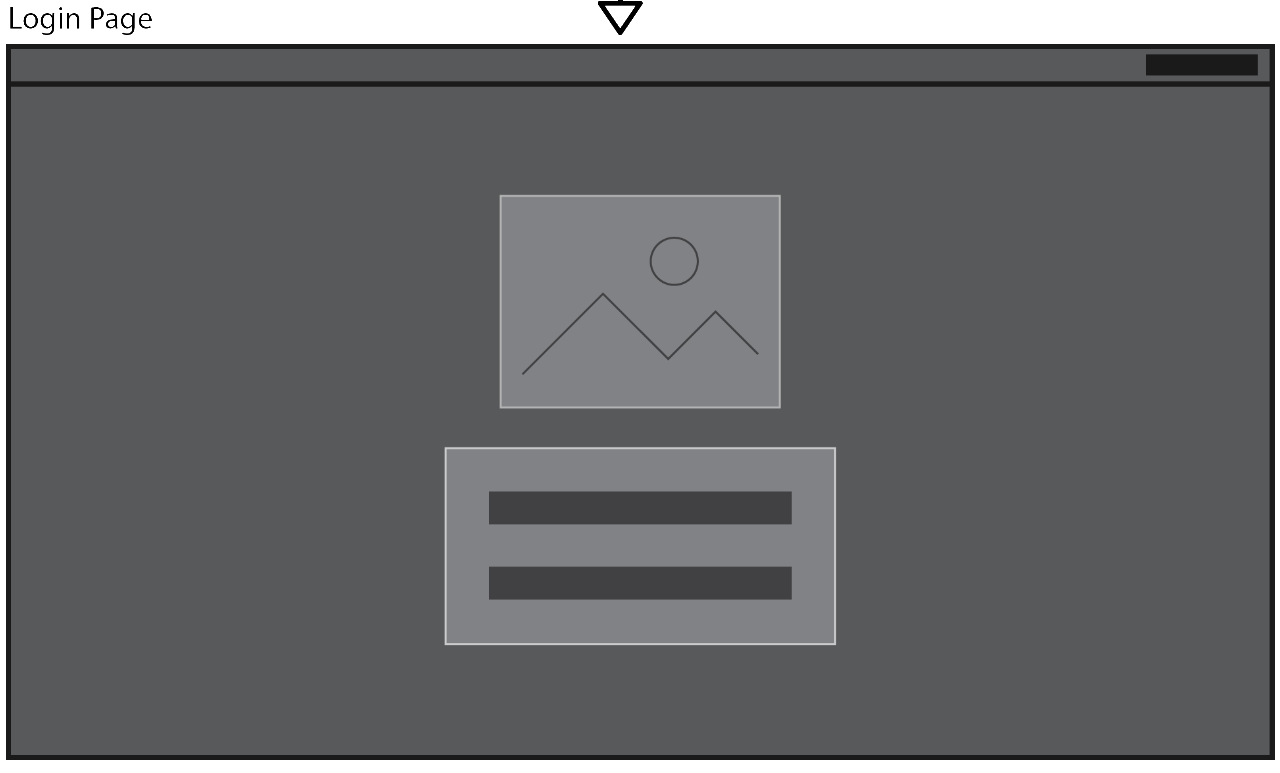
\includegraphics[width=\textwidth]{SoftwareDesign/MVVMDesigns/Graphics/LoginWireframe.png}
    \caption{Wireframe af login}
    \label{fig:LoginWireframe}
\end{figure}

Ud fra Wireframet i figur \ref{fig:LoginWireframe} kan der ses layoutet af Viewet. Det overordnede wireframe viser funktionalitet angående navigation, mellem Views. LoginView skal kun navigere til startpage og til UsersignupView. View'et skal navigere videre til startpage, hvis brugeren logger ind med en oprettet konto. Hvis Brugeen ikke har en konto, trykker brugeren på knappen, som tillader brugeren at oprette en konto, og derved bliver navigeret til Usersignup page.


\subsection{Design af Viewmodel til Login}
Når en bruger prøver at logge ind på sin konto, skal brugerens information overholde nogen regler, som f.eks at det skal være x antal langt kodeord, før det kan godkendes til at være et gyldigt kodeord. Der er et antal validering af brugerens kodeord og email, hvor hvis de ikke bliver overholdt, bliver det udskrevet til brugeren hvilken af brugerens information ikke blev godekendt. Brugerens kodeord er forutroligt information, så det skal ikkee kunne ses i applikationen, så som løsning blev der benyttet securestring til koden, yderlig information af hvordan det fungerer kan ses på \textbf{UserSignUp}. ------- Mangler REF ----------. Der bliver navigeret hen til Start page og Usersignup page via delegate commands.    




\end{document}